% Provenance (never printed): see sources/outline_sources.md (Year 2: radiogenic tracers
% Sr, Nd, Pb and mantle reservoirs; crustal growth; stable isotopes, delta notation and
% fractionation, d18O and d13C). Curves from figdata/bachelor-2/isotopes.py; exercise and
% problem values in the Book 4 scratch calculators calc/ch04.py and calc/ch04pb.py.
% Ruling (Sync 2): delta value and fractionation factor are chemistry's (Year 3 volume),
% recalled; this chapter defines the reference standards and the meteoric water line.
\chapter{Geokimia Isotop}\label{ch:b2:isotope-geochemistry}

Mangaia, di Pasifik selatan, dan Tristan da Cunha, di Atlantik
selatan, sama-sama pulau gunung api yang tersusun atas basal, dan sebuah spesimen tangan dari
yang satu tampak sangat mirip dengan spesimen tangan dari yang lain, atau dari punggungan tengah samudra.
Isotopnya yang membedakan keduanya. Stronsium basal Mangaia membawa
proporsi stronsium-87 yang sama dengan stronsium punggungan, sekitar
$^{87}\mathrm{Sr}/^{86}\mathrm{Sr} = 0.7028$, sedangkan timbalnya termasuk yang paling
radiogenik di Bumi, dengan $^{206}\mathrm{Pb}/^{204}\mathrm{Pb}$ mendekati 21.6 dibandingkan
18.4 untuk punggungan. Basal Tristan memuat lebih banyak stronsium-87, 0.7050 hingga
0.7054, dan lebih sedikit neodimium-143 daripada keduanya. Peleburan tidak memilah isotop
unsur-unsur berat ini, sehingga setiap lava membawa ciri isotop
mantel yang melebur untuk membentuknya: mantel Bumi bukan satu reservoir, melainkan
beberapa, yang telah mempertahankan perbandingan induk--anak yang berbeda selama miliaran
tahun. Bab ini memakai peluruhan radioaktif rubidium, samarium, uranium,
dan torium sebagai seperangkat pelacak, mengikuti evolusi mantel dan
kerak benua melalui isotop neodimium, memisahkan mantel menjadi
reservoir-reservoir dan campuran reservoir, membahas seberapa cepat benua tumbuh,
dan diakhiri dengan isotop stabil ringan oksigen, hidrogen, dan karbon, yang
melacak air dan karbon di dalam Bumi.
% ledger: data:b4-oib-isotopes, gale13:isotopes

\begin{recall}
Induk radioaktif meluruh dengan laju $\lambda P$, dan dalam sistem tertutup
perbandingan anak bertambah sebagai $(D/D_s)_{\text{kini}} = (D/D_s)_0 + (P/D_s)_{\text{kini}}
(e^{\lambda t}-1)$, dengan $D_s$ isotop stabil unsur anak; mineral atau
batuan yang terbentuk bersamaan terletak pada sebuah isokron, yang kemiringannya memberikan umur dan
titik potongnya memberikan perbandingan awal (volume sekolah menengah atas, tahun terakhir; volume Tahun 1,
bab penanggalan radiometrik). Spektrometer massa memisahkan ion menurut
perbandingan massa terhadap muatannya (volume Tahun 2 buku kimia). Nilai $\delta$ sebuah
sampel adalah $\delta = (R_{\text{sampel}}/R_{\text{standar}} - 1)\times 1000$, dalam
permil, dan faktor fraksinasi antara dua fase A dan B adalah
$\alpha_{\mathrm{A/B}} = R_{\mathrm A}/R_{\mathrm B}$, dengan $R$ perbandingan isotop
berat terhadap isotop ringan; keduanya diperkenalkan, bersama energi titik nol
yang menyebabkan fraksinasi isotop, dalam volume Tahun 3 buku kimia.
\omterm{def:b2:elements-in-the-earth:partition}{Unsur inkompatibel}, MORB, dan OIB didefinisikan dalam
\cref{ch:b2:elements-in-the-earth}.
\end{recall}

\section{Isotop radiogenik sebagai pelacak}

Tiga sistem peluruhan membawa sebagian besar informasi tentang mantel dan kerak.
Rubidium-87 meluruh menjadi stronsium-87, samarium-147 menjadi neodimium-143, dan uranium
serta torium, melalui rantai peluruhannya, menjadi tiga isotop timbal. Setiap induk
dan anaknya berbeda perilakunya selama peleburan, dan setiap anak memiliki
isotop stabil non-radiogenik yang menjadi pembanding pengukurannya.

\begin{table}[ht]
\centering
\begin{tabular}{lllll}
\hline
induk & anak & perbandingan terukur & konstanta peluruhan (per tahun) & waktu paruh (Ga)\\
\hline
$^{87}$Rb & $^{87}$Sr & $^{87}\mathrm{Sr}/^{86}\mathrm{Sr}$ & \num{1.3972e-11} & 49.6\\
$^{147}$Sm & $^{143}$Nd & $^{143}\mathrm{Nd}/^{144}\mathrm{Nd}$ & \num{6.524e-12} & 106.25\\
$^{238}$U & $^{206}$Pb & $^{206}\mathrm{Pb}/^{204}\mathrm{Pb}$ & \num{1.55125e-10} & 4.47\\
\hline
\end{tabular}
\caption{Tiga sistem peluruhan berumur panjang yang dipakai sebagai pelacak. Data: rekomendasi
IUPAC--IUGS (Villa dan kawan-kawan, 2020 dan 2022).}
\label{tab:b2:isotope-geochemistry:decay}
\end{table}
% ledger: villa22:rb87, villa20:sm147

\begin{definition}[Pelacak isotop radiogenik]\label{def:b2:isotope-geochemistry:tracer}
Yang disebut \emph{pelacak isotop radiogenik}\index{pelacak isotop radiogenik} adalah perbandingan
isotop anak yang dihasilkan induk radioaktif berumur panjang terhadap isotop stabil
unsur yang sama, seperti $^{87}\mathrm{Sr}/^{86}\mathrm{Sr}$ atau
$^{143}\mathrm{Nd}/^{144}\mathrm{Nd}$, yang dipakai untuk mengenali sumber sebuah batuan alih-alih
untuk menentukan umurnya. Perbandingan sebuah reservoir bertambah dengan laju yang ditentukan oleh
perbandingan induk--anaknya, sehingga merekam sejarah perbandingan itu.
\end{definition}

Kedua unsur sebuah pasangan peluruhan terpisah setiap kali mantel melebur. Pada
\cref{ch:b2:elements-in-the-earth}, rubidium terbukti lebih inkompatibel daripada
stronsium dan neodimium lebih inkompatibel daripada samarium. Lelehan, dan kerak
yang dibangunnya, karena itu meninggalkan mantel dengan Rb/Sr tinggi dan Sm/Nd rendah;
residunya mempertahankan Rb/Sr rendah dan Sm/Nd tinggi. Seiring waktu kerak memperoleh
stronsium-87 lebih cepat daripada sumbernya dan neodimium-143 lebih lambat; \omterm{def:b2:isotope-geochemistry:reservoirs}{mantel
terkuras} berlaku sebaliknya. Perbandingan kedua pasangan bergerak ke arah
yang berlawanan, hal yang diperjelas oleh diagram Sr--Nd di bawah.

\begin{proposition}[Perbandingan isotop bertahan melewati peleburan]\label{prop:b2:isotope-geochemistry:melting}
Ketika sebuah batuan melebur dan lelehannya terpisah dari residu, perbandingan
$^{87}\mathrm{Sr}/^{86}\mathrm{Sr}$ dan $^{143}\mathrm{Nd}/^{144}\mathrm{Nd}$
lelehan sama dengan perbandingan sumbernya dalam batas ketelitian
pengukuran; hanya perbandingan induk--anak, Rb/Sr dan Sm/Nd, yang berubah.
\end{proposition}
\admitted

\noindent Pernyataan itu bertumpu pada dua fakta. Isotop-isotop satu unsur memiliki
struktur elektron yang sama, sehingga masuk ke kristal atau lelehan dengan kemudahan yang hampir sama;
selisih massa relatif antara stronsium-87 dan stronsium-86, sekitar satu
persen, jauh lebih kecil daripada untuk oksigen atau hidrogen, dan pada suhu tinggi
logaritma faktor fraksinasi kesetimbangan turun sebagai kebalikan kuadrat
suhu, mendekati 1. Selain itu, pengukurannya sendiri mengoreksi
fraksinasi yang terjadi di dalam spektrometer massa dengan menetapkan perbandingan dua
isotop non-radiogenik (untuk neodimium, $^{146}\mathrm{Nd}/^{144}\mathrm{Nd} =
0.7219$), yang juga akan menghapus fraksinasi alami yang kecil. Sebuah lava,
karena itu, mencuplik perbandingan isotop sumbernya, sedangkan perbandingan
\omterm{def:b2:elements-in-the-earth:trace}{unsur jejaknya} juga mencerminkan peleburan.
% ledger: white:chur, white:t-dependence

\section{Evolusi mantel dan kerak}

\subsection{Reservoir kondritik}

Samarium dan neodimium sama-sama tanah jarang litofil refraktori
(\cref{ch:b2:elements-in-the-earth}): \omterm{def:b2:elements-in-the-earth:bse}{Bumi silikat total} semestinya mempertahankan
perbandingan kondritiknya. \omterm{def:b2:planet-formation-meteorites:chondrule}{Kondrit} karena itu memberikan sejarah Sm--Nd
Bumi yang belum terdiferensiasi.

\begin{definition}[Reservoir seragam kondritik]\label{def:b2:isotope-geochemistry:chur}
Yang disebut \emph{reservoir seragam kondritik}\index{reservoir seragam kondritik}
(CHUR) adalah reservoir model dengan komposisi samarium--neodimium
\omterm{def:b2:planet-formation-meteorites:chondrule}{kondrit}, yang tertutup sejak pembentukan Tata Surya. Perbandingannya
saat ini adalah $(^{143}\mathrm{Nd}/^{144}\mathrm{Nd})_{\mathrm{CHUR}} = 0.512638$ dan
$(^{147}\mathrm{Sm}/^{144}\mathrm{Nd})_{\mathrm{CHUR}} = 0.1966$.
\end{definition}
% ledger: white:chur

Dihitung mundur dengan persamaan isokron, CHUR memiliki, ketika padatan pertama
mengembun \qty{4567}{Ma} yang lalu (\cref{ch:b2:planet-formation-meteorites}),
\[
  ^{143}\mathrm{Nd}/^{144}\mathrm{Nd} = 0.512638 - 0.1966\,\bigl(e^{\lambda\cdot
  \num{4.567e9}\,\mathrm{yr}}-1\bigr) = 0.506692 .
\] Sejak itu perbandingannya telah bertambah
1.2 persen. Perbedaan antara batuan-batuan Bumi seribu kali lebih
kecil, dan dinyatakan dalam satuan yang lebih praktis.
% ledger: lugaro:cai, villa20:sm147

\begin{definition}[Notasi epsilon]\label{def:b2:isotope-geochemistry:epsilon}
Yang disebut \emph{notasi epsilon}\index{notasi epsilon} menyatakan perbandingan
$^{143}\mathrm{Nd}/^{144}\mathrm{Nd}$ sebuah sampel, pada waktu $t$ sebelum
sekarang, sebagai simpangan relatifnya dari CHUR pada waktu yang sama, dalam bagian per sepuluh
ribu:
\[
  \varepsilon_{\mathrm{Nd}}(t) = \left(
  \frac{(^{143}\mathrm{Nd}/^{144}\mathrm{Nd})_{\text{sampel}}(t)}
       {(^{143}\mathrm{Nd}/^{144}\mathrm{Nd})_{\mathrm{CHUR}}(t)} - 1\right)\times 10^4 .
\]
Tanpa keterangan waktu, $\varepsilon_{\mathrm{Nd}}$ adalah nilai saat ini.
\end{definition}

MORB rata-rata, dengan $^{143}\mathrm{Nd}/^{144}\mathrm{Nd} = 0.513074$, memiliki
$\varepsilon_{\mathrm{Nd}} = (0.513074/0.512638 - 1)\times10^4 = +8.5$; sebagian besar batuan
terletak antara $-20$ dan $+10$. Nilai positif berarti sumber batuan itu
telah memiliki, rata-rata sepanjang sejarah Bumi, Sm/Nd yang lebih tinggi daripada
\omterm{def:b2:planet-formation-meteorites:chondrule}{kondrit}: sumber itu terkuras dalam unsur yang lebih inkompatibel, yaitu neodimium.
Nilai negatif berarti sebaliknya. Penyimpangan dari Sm/Nd kondritik diukur dengan
simpangan fraksional
\[
  f_{\mathrm{Sm/Nd}} = \frac{(\mathrm{Sm}/\mathrm{Nd})_{\text{sampel}}}
  {(\mathrm{Sm}/\mathrm{Nd})_{\mathrm{CHUR}}} - 1,
\]
yang nilainya sama, baik perbandingannya menurut massa maupun menurut atom. Dengan nilai CI
pada \cref{ch:b2:elements-in-the-earth} (Sm 0.145, Nd \qty{0.457}{ppm},
$\mathrm{Sm}/\mathrm{Nd} = 0.317$), kerak benua atas (4.7 dan
\qty{27}{ppm}, 0.174) memiliki $f_{\mathrm{Sm/Nd}} = -0.45$.
% ledger: gale13:isotopes, white:chur, lodders:ci-table, rg03:ucc-trace

\begin{proposition}[Pertumbuhan linear $\varepsilon_{\mathrm{Nd}}$]\label{prop:b2:isotope-geochemistry:linear}
Sebuah reservoir yang terpisah dari CHUR dan sejak itu mempertahankan simpangan fraksional
$f_{\mathrm{Sm/Nd}}$ mengubah $\varepsilon_{\mathrm{Nd}}$-nya, maju dalam
waktu, dengan laju
\[
  \frac{\mathrm{d}\varepsilon_{\mathrm{Nd}}}{\mathrm{d}\tau} \approx Q\,f_{\mathrm{Sm/Nd}},
  \qquad
  Q = 10^4\,\lambda_{147}\,
  \frac{(^{147}\mathrm{Sm}/^{144}\mathrm{Nd})_{\mathrm{CHUR}}}
       {(^{143}\mathrm{Nd}/^{144}\mathrm{Nd})_{\mathrm{CHUR}}}
  = \qty{25.0}{\per\Ga},
\]
dengan $\tau$ waktu yang dihitung maju. Sebuah reservoir dengan $\varepsilon_0$ pada saat
pemisahannya, waktu $T$ yang lalu, kini memiliki $\varepsilon_{\mathrm{Nd}} \approx \varepsilon_0
+ Q f_{\mathrm{Sm/Nd}} T$.
\end{proposition}

\begin{proof}
Tuliskan $R$ untuk $^{143}\mathrm{Nd}/^{144}\mathrm{Nd}$ dan $p$ untuk
$^{147}\mathrm{Sm}/^{144}\mathrm{Nd}$. Dalam reservoir tertutup
$\mathrm{d}R/\mathrm{d}\tau = \lambda p\,e^{\lambda t}$, dengan $t$ waktu sebelum
sekarang; karena $\lambda t \le 0.03$, faktor $e^{\lambda t}$ berbeda dari 1 paling
banyak 3 persen, dan $\mathrm{d}R/\mathrm{d}\tau \approx \lambda p$. Maka
$\mathrm{d}(R_s - R_c)/\mathrm{d}\tau \approx \lambda (p_s - p_c) = \lambda p_c
f_{\mathrm{Sm/Nd}}$, karena $p_s/p_c - 1 = f_{\mathrm{Sm/Nd}}$. Membagi dengan $R_c$,
yang hanya berubah 1.2 persen sepanjang umur Bumi, menghasilkan
$\mathrm{d}\varepsilon/\mathrm{d}\tau \approx 10^4\lambda p_c f/R_c$. Dengan
$\lambda = \qty{6.524e-12}{\per\year}$, $p_c = 0.1966$, dan $R_c = 0.512638$, $Q =
\num{2.502e-8}$ per tahun, \qty{25.0}{\per\Ga}.
\end{proof}
% ledger: villa20:sm147, white:chur

Kerak dengan Sm/Nd kerak atas ($f = -0.45$) karena itu kehilangan sekitar
11 satuan epsilon per miliar tahun relatif terhadap CHUR, sedangkan reservoir mantel
hanya memerlukan $f = +0.07$ untuk naik dari 0 ke nilai MORB $+8.5$ dalam
\qty{4.567}{Ga}. Gambar di bawah mengikuti persamaan eksak untuk tiga
reservoir: CHUR, \omterm{def:b2:isotope-geochemistry:reservoirs}{mantel terkuras} yang tertutup sejak Bumi terbentuk dengan Sm/Nd
yang membawanya ke nilai MORB saat ini ($^{147}\mathrm{Sm}/^{144}\mathrm{Nd} =
0.211$), dan kerak yang diekstraksi dari mantel itu 2.7 miliar tahun yang lalu dengan
Sm/Nd kerak atas ($0.108$). Kerak itu bermula pada $\varepsilon_{\mathrm{Nd}} =
+3.5$, nilai sumbernya pada waktu itu, dan kini berada pada $-27$.

\begin{definition}[Mantel terkuras, mantel diperkaya]\label{def:b2:isotope-geochemistry:reservoirs}
Yang disebut \emph{mantel terkuras}\index{mantel terkuras} adalah bagian mantel yang telah
kehilangan \omterm{def:b2:elements-in-the-earth:partition}{unsur inkompatibel} ke dalam lelehan, sehingga Sm/Nd-nya lebih tinggi dan Rb/Sr-nya
lebih rendah daripada kondritik; seiring waktu $\varepsilon_{\mathrm{Nd}}$-nya menjadi positif dan
$^{87}\mathrm{Sr}/^{86}\mathrm{Sr}$-nya rendah. Yang disebut \emph{mantel
diperkaya}\index{mantel diperkaya} adalah bagian mantel yang telah memperoleh
\omterm{def:b2:elements-in-the-earth:partition}{unsur inkompatibel}, misalnya dari kerak yang didaur ulang atau dari lelehan kecil,
dengan $\varepsilon_{\mathrm{Nd}}$ negatif atau $^{87}\mathrm{Sr}/^{86}\mathrm{Sr}$ tinggi.
\end{definition}

\begin{omfigure}
\centering
\begin{tikzpicture}
\begin{axis}[omrecord, width=0.82\linewidth, height=6.4cm,
  x dir=reverse, xmin=0, xmax=4.6, ymin=-30, ymax=12,
  xlabel={waktu sebelum sekarang (Ga)}, ylabel={$\varepsilon_{\mathrm{Nd}}(t)$},
  tick label style={font=\scriptsize}, label style={font=\small}]
\addplot[thick, black] table[x=t_Ga, y=eps] {figdata/out/bachelor-2-isotopes-chur.dat};
\addplot[very thick, blue!70!black] table[x=t_Ga, y=eps] {figdata/out/bachelor-2-isotopes-dm.dat};
\addplot[very thick, brown!70!black] table[x=t_Ga, y=eps] {figdata/out/bachelor-2-isotopes-crust.dat};
\addplot[densely dashed, gray] coordinates {(2.7,-30) (2.7,12)};
\node[font=\scriptsize, anchor=north] at (axis cs:3.6,-0.6) {CHUR};
\node[font=\scriptsize, blue!70!black, anchor=south east] at (axis cs:0.4,8.8) {mantel terkuras, $+8.5$};
\node[font=\scriptsize, brown!70!black, anchor=north east] at (axis cs:0.3,-25.5) {kerak, $-27$};
\node[font=\scriptsize, gray, anchor=north west, align=left] at (axis cs:2.65,-12) {kerak diekstraksi\\pada \qty{2.7}{Ga}};
\end{axis}
\end{tikzpicture}
\par\smallskip{\small Evolusi isotop neodimium, sebagai $\varepsilon_{\mathrm{Nd}}$, dari
reservoir kondritik (nol menurut definisi), dari \omterm{def:b2:isotope-geochemistry:reservoirs}{mantel terkuras} yang tertutup sejak
\qty{4.567}{Ga} yang Sm/Nd-nya membawanya ke MORB rata-rata saat ini, dan dari kerak yang
diekstraksi darinya \qty{2.7}{Ga} yang lalu dengan Sm/Nd kerak benua
atas. Setiap garis hampir lurus, seperti dikatakan proposisi pertumbuhan linear. Data:
CHUR, buku teks White; MORB rata-rata, Gale dan kawan-kawan (2013); Sm/Nd kerak,
Rudnick dan Gao.}
\end{omfigure}
% ledger: white:chur, villa20:sm147, gale13:isotopes, rg03:ucc-trace, lodders:ci-table, lugaro:cai

\subsection{Dua reservoir yang saling melengkapi}

Jika kerak benua dan \omterm{def:b2:isotope-geochemistry:reservoirs}{mantel terkuras} dibuat dari satu reservoir
kondritik, neodimium keduanya harus dijumlahkan kembali menjadi nilai kondritik. Neodimium adalah
pembawanya: setiap reservoir dihitung sebanding dengan neodimium yang dimuatnya.

\begin{proposition}[Neraca massa isotop]\label{prop:b2:isotope-geochemistry:mass-balance}
Misalkan reservoir-reservoir $i$ bermassa $M_i$ dengan konsentrasi neodimium $C_i$ berasal dari
pembagian satu reservoir induk. Maka, dengan pendekatan yang sangat baik,
\[
  \sum_i M_i C_i\, \varepsilon_i = \Bigl(\sum_i M_i C_i\Bigr) \varepsilon_{\text{induk}},
\]
kedua ruas dievaluasi pada waktu yang sama, dan induknya diikuti seolah-olah
tetap utuh.
\end{proposition}

\begin{proof}
Jumlah atom $^{143}\mathrm{Nd}$ dan jumlah atom $^{144}\mathrm{Nd}$
masing-masing kekal dalam pembagian itu, dan masing-masing kemudian bertambah (untuk
$^{143}\mathrm{Nd}$) atau tetap (untuk $^{144}\mathrm{Nd}$) di setiap reservoir tepat seperti
dalam keseluruhannya. Karena itu rata-rata berbobot-$^{144}\mathrm{Nd}$ perbandingan $R_i$ sama dengan
perbandingan induk, $R_p$. Bagian $^{144}\mathrm{Nd}$ dalam neodimium bervariasi
antarreservoir jauh kurang dari satu per seribu, sehingga pembobotan dengan
$M_iC_i$ sama dengan pembobotan dengan $^{144}\mathrm{Nd}$. Akhirnya $\varepsilon$ adalah
fungsi linear $R$ pada waktu tertentu, $\varepsilon = 10^4(R/R_c - 1)$, dan
rata-rata berbobot fungsi-fungsi linear adalah fungsi linear dari rata-rata berbobotnya.
\end{proof}

Dengan nilai kerak atas \qty{27}{ppm} neodimium yang diambil untuk seluruh
kerak, kerak benua sebesar \qty{7.2e9}{km^3} dengan \qty{2830}{kg/m^3}, yaitu
\qty{2.0e22}{kg} atau 0.51 persen massa Bumi silikat, memuat
$0.0051\times27/1.25 = 11$ persen neodimium Bumi silikat (\omterm{def:b2:elements-in-the-earth:bse}{mantel
primitif}, \qty{1.25}{ppm}). Jika kerak memiliki $\varepsilon_{\mathrm{Nd}}$ rata-rata
$-15$, sumbangan negatif sebesar $0.11\times15 = 1.65$ satuan harus
diimbangi oleh mantel: reservoir pada nilai MORB $+8.5$ harus memuat
sekitar seperlima neodimium Bumi silikat (\cref{exo:b2:isotope-geochemistry:9}). Inilah salah satu
argumen bahwa \omterm{def:b2:isotope-geochemistry:reservoirs}{mantel terkuras} yang dicuplik punggungan bukanlah seluruh
mantel.
% ledger: cogley84:continents, cm95:crust, ms95:pm-trace, rg03:ucc-trace, data:prem, earth:mass, gale13:isotopes

\section{Reservoir-reservoir mantel}

Perbandingan isotop basal samudra mencuplik mantel tanpa melewati
kerak benua. Jika diplot satu terhadap yang lain, perbandingan itu menunjukkan
sifat saling melengkapi kerak dan \omterm{def:b2:isotope-geochemistry:reservoirs}{mantel terkuras} sekaligus keberadaan reservoir
lain.

Isotop stronsium dan neodimium berkorelasi negatif pada sebagian besar basal samudra:
lava dengan $\varepsilon_{\mathrm{Nd}}$ tinggi memiliki
$^{87}\mathrm{Sr}/^{86}\mathrm{Sr}$ rendah. Pita ini disebut larik mantel; pita itu timbul
dari perilaku yang berlawanan kedua pasangan selama peleburan (rubidium kurang
kompatibel daripada stronsium, samarium lebih kompatibel daripada neodimium). MORB
rata-rata terletak di ujungnya yang terkuras, dengan $^{87}\mathrm{Sr}/^{86}\mathrm{Sr} = 0.702819$ dan
$\varepsilon_{\mathrm{Nd}} = +8.5$. \omterm{def:b2:elements-in-the-earth:morb-oib}{Basal pulau samudra} menyebar dari situ ke arah
$\varepsilon_{\mathrm{Nd}}$ yang lebih rendah dan $^{87}\mathrm{Sr}/^{86}\mathrm{Sr}$ yang lebih tinggi, tetapi tidak
sepanjang satu garis.
% ledger: white:dm, gale13:isotopes

\begin{definition}[Anggota ujung mantel]\label{def:b2:isotope-geochemistry:end-members}
Yang disebut \emph{anggota ujung mantel}\index{anggota ujung mantel} adalah salah satu komposisi
isotop ekstrem yang darinya perbandingan isotop Sr, Nd, dan Pb basal
samudra dapat dibangun melalui pencampuran. Empat yang umum dinamai: DMM, mantel
MORB yang terkuras (depleted MORB mantle; $^{87}\mathrm{Sr}/^{86}\mathrm{Sr}$ rendah, $\varepsilon_{\mathrm{Nd}}$ tinggi);
HIMU, untuk $\mu = {}^{238}\mathrm{U}/^{204}\mathrm{Pb}$ yang tinggi di sumbernya
(timbal yang sangat radiogenik, $^{206}\mathrm{Pb}/^{204}\mathrm{Pb}$ di atas 20, dengan
$^{87}\mathrm{Sr}/^{86}\mathrm{Sr}$ rendah); EM1, \omterm{def:b2:isotope-geochemistry:reservoirs}{mantel diperkaya} 1 (enriched mantle 1; $^{87}\mathrm{Sr}/^{86}\mathrm{Sr}$
cukup tinggi, $\varepsilon_{\mathrm{Nd}}$ negatif, timbal tidak
radiogenik); dan EM2, \omterm{def:b2:isotope-geochemistry:reservoirs}{mantel diperkaya} 2 ($^{87}\mathrm{Sr}/^{86}\mathrm{Sr}$ tinggi).
\end{definition}
% ledger: white:end-members

\begin{omfigure}
\centering
\begin{tikzpicture}
\begin{axis}[omrecord, width=0.82\linewidth, height=6.6cm,
  xmin=0.7020, xmax=0.7064, ymin=-6, ymax=11,
  xlabel={$^{87}\mathrm{Sr}/^{86}\mathrm{Sr}$}, ylabel={$\varepsilon_{\mathrm{Nd}}$},
  xticklabel style={/pgf/number format/fixed, /pgf/number format/precision=4},
  scaled x ticks=false, legend pos=south west, legend cell align=left,
  legend style={font=\scriptsize}, tick label style={font=\scriptsize},
  label style={font=\small}]
\addplot[only marks, mark=*, mark size=1.3pt, red!70!black] table[x=sr, y=eps] {figdata/out/bachelor-2-isotopes-himu.dat};
\addlegendentry{tipe HIMU: St.\ Helena, Mangaia, Tubuai}
\addplot[only marks, mark=square*, mark size=1.2pt, brown!70!black] table[x=sr, y=eps] {figdata/out/bachelor-2-isotopes-em1.dat};
\addlegendentry{tipe EM1: Tristan da Cunha, Gough}
\addplot[only marks, mark=diamond*, mark size=3pt, blue!70!black] table[x=sr, y=eps] {figdata/out/bachelor-2-isotopes-morb.dat};
\addlegendentry{MORB rata-rata}
\addplot[densely dashed, gray] coordinates {(0.7020,0) (0.7064,0)};
\node[font=\scriptsize, gray, anchor=south east] at (axis cs:0.7063,0.1) {CHUR};
\draw[->, gray] (axis cs:0.7030,9.5) -- (axis cs:0.7046,0.8);
\node[font=\scriptsize, gray, anchor=west, align=left] at (axis cs:0.7036,6.5) {larik mantel:\\terkuras ke diperkaya};
\end{axis}
\end{tikzpicture}
\par\smallskip{\small Isotop stronsium dan neodimium 89 basal dari lima
pulau samudra dan \omterm{def:b2:elements-in-the-earth:morb-oib}{basal punggungan tengah samudra} rata-rata. Pulau-pulau tipe HIMU terplot
di bawah larik utama, dengan perbandingan stronsium MORB yang rendah tetapi
$\varepsilon_{\mathrm{Nd}}$ yang lebih rendah; pulau-pulau tipe EM1 terletak di sisi CHUR yang diperkaya.
Lava Samoa tipe EM2 mencapai $^{87}\mathrm{Sr}/^{86}\mathrm{Sr} = 0.7205$, jauh
di luar skala ini di sebelah kanan. Data: Stracke dan kawan-kawan (2022), CC BY 4.0; Gale dan
kawan-kawan (2013); Edwards dan kawan-kawan (2019).}
\end{omfigure}
% ledger: data:b4-oib-isotopes, gale13:isotopes, edwards19:samoa, white:chur

Kelompok-kelompok pulau pada gambar di atas tidak acak. Kelompok St.~Helena,
yang mencakup Kepulauan Austral (di antaranya Mangaia dan Tubuai) dan
Ascension, terplot di bawah larik utama dan memiliki timbal yang paling radiogenik
($^{206}\mathrm{Pb}/^{204}\mathrm{Pb}$ di atas 20; Mangaia mencapai 21.5 hingga 22.0).
Kelompok Kerguelen, yaitu Tristan da Cunha, Gough, dan Kerguelen, terletak pada
$^{87}\mathrm{Sr}/^{86}\mathrm{Sr}$ cukup tinggi dan $\varepsilon_{\mathrm{Nd}}$ negatif, selalu dengan
timbal yang tidak radiogenik. Kelompok Society, bersama Samoa dan Marquesas, membentuk
tren Sr--Nd yang lebih landai hingga perbandingan stronsium yang sangat tinggi: dua lava Samoa
memiliki $^{87}\mathrm{Sr}/^{86}\mathrm{Sr}$ 0.7186 dan 0.7205, lebih tinggi daripada air laut
modern (0.7092). Kelompok St.~Helena, Kerguelen, dan Society adalah tipe HIMU,
EM1, dan EM2.
% ledger: white:end-members, data:b4-oib-isotopes, edwards19:samoa

Perbandingan yang berbeda antara dua bagian mantel pasti telah
dipertahankan oleh perbedaan perbandingan induk--anak dalam waktu yang lama: perbedaan
10 satuan $\varepsilon_{\mathrm{Nd}}$ memerlukan, menurut proposisi pertumbuhan
linear, 1 miliar tahun pada $f = 0.4$ atau 4 miliar tahun pada $f = 0.1$. Reservoir-reservoir
mantel karena itu sudah tua. Hakikatnya dibaca dari
perbandingan induk--anak yang dituntut isotopnya. HIMU memerlukan U/Pb tinggi dan
Rb/Sr rendah dalam waktu yang lama, yang cocok dengan kerak samudra yang kehilangan timbal dan rubidium
dalam fluida yang dilepaskan di atas zona subduksi lalu tersimpan di dalam mantel
selama satu atau dua miliar tahun. EM1 dan EM2 memerlukan Sm/Nd rendah dan, untuk EM2,
Rb/Sr tinggi: ciri bahan yang berasal dari benua, seperti sedimen
yang didaur ulang, atau mantel yang diperkaya oleh lelehan kecil. Tafsiran-tafsiran ini
masih diperdebatkan; pengukurannya tidak.
% ledger: white:end-members

\begin{omfigure}
\centering
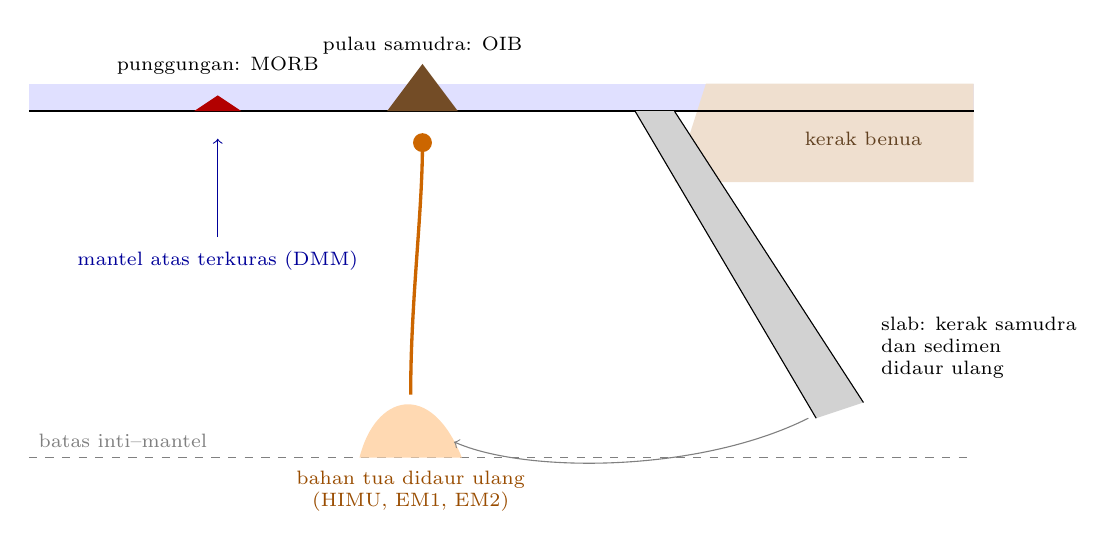
\begin{tikzpicture}[x=1cm, y=1cm, font=\scriptsize]
  % surface and lithosphere
  \fill[blue!12] (-6,0) rectangle (6,0.35);
  \fill[brown!25] (2.6,0.35) -- (6,0.35) -- (6,-0.9) -- (2.2,-0.9) -- cycle;
  \node[brown!50!black] at (4.6,-0.35) {kerak benua};
  \draw[thick] (-6,0) -- (6,0);
  % ridge
  \node[anchor=south] at (-3.6,0.35) {punggungan: MORB};
  \draw[->, blue!60!black] (-3.6,-1.6) -- (-3.6,-0.35);
  \node[blue!60!black, anchor=north] at (-3.6,-1.65) {mantel atas terkuras (DMM)};
  % slab
  \fill[gray!35] (1.7,0) -- (2.2,0) -- (4.6,-3.7) -- (4.0,-3.9) -- cycle;
  \draw (1.7,0) -- (4.0,-3.9) (2.2,0) -- (4.6,-3.7);
  \node[anchor=west, align=left] at (4.7,-3.0) {slab: kerak samudra\\dan sedimen\\didaur ulang};
  % deep pool and plume
  \draw[gray, dashed] (-6,-4.4) -- (6,-4.4);
  \node[anchor=south west, gray] at (-6,-4.4) {batas inti--mantel};
  \fill[orange!30] (-1.8,-4.4) .. controls (-1.6,-3.6) and (-0.9,-3.4) .. (-0.5,-4.4) -- cycle;
  \draw[very thick, orange!80!black] (-1.15,-3.6) .. controls (-1.15,-2.4) and (-1.0,-1.3) .. (-1.0,-0.4);
  \fill[orange!80!black] (-1.0,-0.4) circle (0.12);
  \fill[brown!60!black] (-1.45,0) -- (-1.0,0.6) -- (-0.55,0) -- cycle;
  \node[anchor=south] at (-1.0,0.6) {pulau samudra: OIB};
  \fill[red!70!black] (-3.9,0) -- (-3.6,0.2) -- (-3.3,0) -- cycle;
  \node[orange!60!black, anchor=north, align=center] at (-1.15,-4.45) {bahan tua didaur ulang\\(HIMU, EM1, EM2)};
  \draw[->, gray] (3.9,-3.9) .. controls (2.5,-4.6) and (0.3,-4.6) .. (-0.6,-4.2);
\end{tikzpicture}
\par\smallskip{\small Salah satu tafsiran reservoir mantel yang banyak dipakai, tidak menurut
skala: punggungan mencuplik mantel atas yang terkuras; kerak samudra dan sedimen
kembali ke mantel di zona subduksi; plume yang naik dari mantel dalam
membawa ke atas bahan yang di dalamnya komponen tua yang didaur ulang bercampur, dan memberi
pulau-pulau itu sifat HIMU, EM1, atau EM2-nya.}
\end{omfigure}

\section{Pencampuran}

Banyak larik isotop merupakan campuran. Sebuah lava dapat berasal dari sumber yang merupakan
campuran dua reservoir, atau sebuah magma dapat menyerap sebagian kerak yang dilewatinya.
Kedua kasus itu mengikuti aljabar yang sama.

\begin{proposition}[Hiperbola pencampuran]\label{prop:b2:isotope-geochemistry:mixing}
Misalkan sebuah campuran mengandung fraksi massa $f$ komponen A dan $1-f$ komponen
B. Untuk sebuah unsur dengan konsentrasi $C_{\mathrm A}$, $C_{\mathrm B}$ dan perbandingan
isotop $R_{\mathrm A}$, $R_{\mathrm B}$:
\begin{enumerate}
\item konsentrasi campuran, $C = fC_{\mathrm A} + (1-f)C_{\mathrm B}$, dan
perbandingan isotopnya,
$R = \bigl(fC_{\mathrm A}R_{\mathrm A} + (1-f)C_{\mathrm B}R_{\mathrm B}\bigr)/C$, memenuhi
$R = a + b/C$ dengan konstanta $a$ dan $b$: campuran-campuran itu terletak pada garis lurus dalam
plot $R$ terhadap $1/C$;
\item dua perbandingan semacam itu dari dua unsur, $R$ dan $R'$, terletak pada sebuah hiperbola, yang disebut
\emph{hiperbola pencampuran}\index{hiperbola pencampuran}, yang berupa garis lurus hanya
jika perbandingan kedua unsur itu sama di A dan B. Kelengkungannya ditentukan oleh
$K = (C'/C)_{\mathrm A}/(C'/C)_{\mathrm B}$.
\end{enumerate}
\end{proposition}

\begin{proof}
(1) Eliminasi $f$: $f = (C - C_{\mathrm B})/(C_{\mathrm A} - C_{\mathrm B})$. Maka
$RC = C_{\mathrm B}R_{\mathrm B} + f(C_{\mathrm A}R_{\mathrm A} - C_{\mathrm B}R_{\mathrm
B})$ linear terhadap $C$, $RC = \alpha + \beta C$, dan $R = \beta + \alpha/C$.
(2) Bagian unsur yang berasal dari A adalah $s = fC_{\mathrm A}/C$, dan $R =
R_{\mathrm B} + s(R_{\mathrm A} - R_{\mathrm B})$ linear terhadap $s$; demikian pula $R'$
linear terhadap $s' = fC'_{\mathrm A}/C'$. Dengan $u = f/(1-f)$, $s = u C_{\mathrm
A}/(uC_{\mathrm A} + C_{\mathrm B})$ dan $s' = uC'_{\mathrm A}/(uC'_{\mathrm A} +
C'_{\mathrm B})$. Mengeliminasi $u$ menghasilkan $s' = Ks/(1 + (K-1)s)$, sebuah hiperbola pada
bidang $(s, s')$, dan karena itu pada bidang $(R, R')$; hiperbola itu menjadi garis lurus $s' = s$
ketika $K = 1$.
\end{proof}

\begin{omfigure}
\centering
\begin{tikzpicture}
\begin{axis}[omrecord, width=0.62\linewidth, height=6.2cm,
  xmin=0, xmax=1, ymin=0, ymax=1,
  xlabel={perbandingan pertama, diskalakan ulang (B $=0$, A $=1$)},
  ylabel={perbandingan kedua, diskalakan ulang},
  tick label style={font=\scriptsize}, label style={font=\small}]
\addplot[thick, red!70!black] table[x=x, y=y] {figdata/out/bachelor-2-isotopes-mixK50.dat};
\addplot[thick, black] table[x=x, y=y] {figdata/out/bachelor-2-isotopes-mixK10.dat};
\addplot[thick, blue!70!black] table[x=x, y=y] {figdata/out/bachelor-2-isotopes-mixK02.dat};
\node[font=\scriptsize, red!70!black, anchor=south east] at (axis cs:0.30,0.72) {$K=5$};
\node[font=\scriptsize, anchor=south east] at (axis cs:0.55,0.56) {$K=1$};
\node[font=\scriptsize, blue!70!black, anchor=north west] at (axis cs:0.62,0.22) {$K=0.2$};
\node[font=\scriptsize, anchor=north west] at (axis cs:0.0,0.0) {B};
\node[font=\scriptsize, anchor=south east] at (axis cs:1.0,1.0) {A};
\end{axis}
\end{tikzpicture}
\par\smallskip{\small Kurva pencampuran antara dua komponen A dan B untuk tiga
nilai $K$, perbandingan kedua unsur di A dibagi perbandingannya di B. Setiap
perbandingan isotop diskalakan ulang menjadi 0 di B dan 1 di A; unsur kedua $K$ kali
lebih kaya di A, relatif terhadap unsur pertama, daripada di B, sehingga perbandingan kedua bergerak menuju
A lebih cepat ketika $K > 1$.}
\end{omfigure}

Komponen yang kaya akan suatu unsur mendominasi perbandingan isotop unsur itu dalam
campuran. Sedimen yang didaur ulang memuat neodimium puluhan kali lebih banyak daripada
\omterm{def:b2:isotope-geochemistry:reservoirs}{mantel terkuras}, dan beberapa persen sedimen itu dalam sumber mantel menarik
$\varepsilon_{\mathrm{Nd}}$ campuran sebagian besar jalan menuju nilainya sendiri (soal).
Pulau-pulau tipe HIMU pada gambar Sr--Nd terletak di luar setiap kurva pencampuran antara MORB
dan pulau-pulau EM1: tidak ada campuran dua komponen yang menjelaskan semua basal samudra,
dan anggota ujungnya sedikitnya empat. Magma yang mengasimilasi kerak
benua bergerak sepanjang kurva pencampuran menuju kerak; posisinya pada kurva
memberikan proporsi kerak yang terserap, perhitungan yang dibahas lagi bersama kristalisasi
pada \cref{ch:b2:magmatic-differentiation}.

\section{Pertumbuhan kerak benua}

Kerak benua adalah pelengkap \omterm{def:b2:isotope-geochemistry:reservoirs}{mantel terkuras}; seberapa cepat kerak itu
diekstraksi adalah salah satu pertanyaan tertua geokimia isotop, dan masih
terbuka. Beberapa rekaman berkaitan dengannya.

\begin{definition}[Kurva pertumbuhan kerak]\label{def:b2:isotope-geochemistry:growth}
Yang disebut \emph{kurva pertumbuhan kerak}\index{kurva pertumbuhan kerak} memberikan volume, atau
massa, kerak benua yang ada sebagai fungsi waktu, sebagai fraksi
volume saat ini. Kurva itu mencerminkan keseimbangan antara pembentukan kerak baru
dari mantel dan penghancurannya melalui daur ulang ke dalam mantel.
\end{definition}

Batuan yang terawetkan saat ini memberikan kurva pertama: kurang dari seperempat volume
kerak benua juvenil yang terawetkan saat ini lebih tua daripada \qty{3}{Ga}, dan
tidak ada batuan yang dikenal dengan umur kristalisasi lebih tua daripada \qty{4.02}{Ga}. Namun
kerak yang terawetkan adalah apa yang bertahan, bukan apa yang dibuat. Kurva-kurva lain dibangun dari
isotop neodimium serpih, yang merata-ratakan kerak atas yang tersingkap terhadap
erosi pada saat serpih itu diendapkan; dari isotop hafnium butir
zirkon, yang merekam apakah magma yang mengkristalkannya berasal dari kerak baru atau
kerak yang diolah ulang; atau dari isotop argon kuarsa hidrotermal, yang melacak
pelepasan gas kerak. Beberapa model terbaru jenis ini menempatkan sedikitnya 60
hingga 80 persen volume kerak benua saat ini sudah terbentuk pada
\qty{3}{Ga}. Kedua pandangan itu hanya dapat didamaikan jika sangat banyak kerak awal
yang dihancurkan: dalam satu model kotak yang dicocokkan dengan kedua rekaman, 2.3 hingga 2.6 kali
volume kerak benua saat ini telah dibentuk sejak Bumi terbentuk,
dan 1.3 hingga 1.6 kali volume itu telah dikembalikan ke mantel.
% ledger: dhuime18:growth

Zona subduksi masa kini memperlihatkan daur ulang itu sedang bekerja. Magmatisme busur menambahkan
sekitar 2.5 kilometer kubik kerak baru per tahun, 1.5 di busur intraoseanik dan
1.0 di tepi benua (2.7 sebagai rata-rata jangka panjang), sedangkan subduksi membawa
kembali sekitar 3.2 kilometer kubik per tahun; dalam batas ketidakpastiannya,
benua tidak tumbuh setidaknya selama Fanerozoikum. Isotop \omterm{def:b2:isotope-geochemistry:end-members}{anggota ujung
mantel}, yang menuntut kerak dan sedimen yang didaur ulang, adalah sisi lain dari
perhitungan yang sama.
% ledger: sv09:growth

\section{Isotop stabil}

Isotop unsur-unsur ringan, yaitu hidrogen, karbon, nitrogen, oksigen, dan
belerang, tidak dihasilkan oleh peluruhan dalam jumlah yang terukur. Isotop-isotop itu justru difraksinasi
oleh proses fisika, kimia, dan biologi, dengan selisih massa relatif
hingga dua kali lipat untuk hidrogen dan deuterium, dan
variasinya dilaporkan sebagai nilai $\delta$ relatif terhadap standar yang disepakati.

\begin{definition}[Standar acuan isotop]\label{def:b2:isotope-geochemistry:standards}
Yang disebut \emph{standar acuan isotop}\index{standar acuan isotop} adalah
bahan yang perbandingan isotopnya menetapkan titik nol sebuah skala $\delta$. Dua di antaranya dipakai
dalam ilmu kebumian. \emph{VSMOW}\index{VSMOW} (yaitu air samudra rata-rata
standar Wina) menetapkan $\delta\mathrm{D}$ dan $\delta^{18}\mathrm{O}$ air, silikat, dan
sebagian besar bahan lain; perbandingan mutlaknya adalah $\mathrm{D}/\mathrm{H} =
\num{1.5575e-4}$ dan $^{18}\mathrm{O}/^{16}\mathrm{O} = \num{2.0052e-3}$.
\emph{VPDB}\index{VPDB} (yaitu belemnit Pee Dee standar Wina) menetapkan $\delta^{13}\mathrm{C}$
dan $\delta^{18}\mathrm{O}$ karbonat bersuhu rendah; perbandingan mutlaknya
adalah $^{13}\mathrm{C}/^{12}\mathrm{C} = \num{1.1237e-2}$ dan
$^{18}\mathrm{O}/^{16}\mathrm{O} = \num{2.0672e-3}$.
\end{definition}
% ledger: kc98:standards

Nama-nama itu mengingatkan pada sejarahnya: SMOW adalah air samudra rata-rata, dan PDB
karbonat fosil belemnit dari formasi Pee Dee; bahan-bahan
aslinya habis dan diganti dengan bahan acuan yang dikalibrasi terhadapnya,
yang didistribusikan oleh Badan Tenaga Atom Internasional di Wina dan oleh NIST.
Pada skala \omterm{def:b2:isotope-geochemistry:standards}{VSMOW}, oksigen \omterm{def:b2:isotope-geochemistry:standards}{VPDB} memiliki $\delta^{18}\mathrm{O} = +30.9$ permil
(\cref{exo:b2:isotope-geochemistry:2}): karbonat laut sebanyak itu lebih berat daripada air samudra tempat karbonat itu
tumbuh.
% ledger: kc98:standards

\subsection{Air}

Air samudra terletak di sekitar $\delta^{18}\mathrm{O} = \delta\mathrm{D} = 0$, menurut
definisi \omterm{def:b2:isotope-geochemistry:standards}{VSMOW}. Penguapan lebih menyukai isotop ringan: dalam kesetimbangan
dengan air cair pada \qty{20}{\degreeCelsius}, dengan faktor fraksinasi
1.0098 untuk oksigen-18 dan 1.084 untuk deuterium, uapnya akan memiliki
$\delta^{18}\mathrm{O} = 1000/1.0098 - 1000 = -9.7$ permil dan $\delta\mathrm{D} =
-77$ permil; uap di atas samudra bahkan lebih ringan, sekitar $-13$ permil
dalam $\delta^{18}\mathrm{O}$, karena penguapan juga merupakan proses kinetik.
Ketika sebuah massa udara bergerak ke pedalaman dan ke arah kutub serta mendingin, massa udara itu menurunkan hujan, dan
setiap hujan mengambil isotop berat lebih dulu; uap yang tersisa, serta hujan dan
salju yang menyusul, menjadi makin lama makin ringan. Es Greenland umumnya memiliki
$\delta^{18}\mathrm{O}$ $-30$ hingga $-35$ permil, es Antarktika serendah $-50$.
% ledger: kc98:alpha, white:d18o

\begin{proposition}[Garis air meteorik]\label{prop:b2:isotope-geochemistry:mwl}
Hujan dan salju dari seluruh dunia, serta air tawar yang berasal darinya,
terletak dekat \emph{garis air meteorik}\index{garis air meteorik}
\[
  \delta\mathrm{D} = 8\,\delta^{18}\mathrm{O} + 10 \quad\text{(permil, VSMOW)},
\]
yang ditetapkan secara empiris oleh Craig pada tahun 1961. Titik potongnya, 10 permil, disebut
kelebihan deuterium; masing-masing wilayah memiliki nilai antara sekitar 0 dan 20.
\end{proposition}
\admitted

\noindent Kemiringannya dapat dipahami tanpa teori kondensasi yang lengkap,
yang diserahkan kepada volume Tahun 3. Pada setiap langkah kondensasi, cairan
dan uap berbeda sekitar $1000(\alpha - 1)$ permil untuk setiap isotop, dan
kedua pergeseran itu berbanding $(\alpha_{\mathrm D}-1)/(\alpha_{18}-1)$, yang
bernilai 8.6 pada \qty{20}{\degreeCelsius} dan 9.5 pada \qty{0}{\degreeCelsius}: ketika
uap terkuras langkah demi langkah, $\delta\mathrm{D}$ turun sekitar delapan kali lebih cepat
daripada $\delta^{18}\mathrm{O}$. Titik potongnya tidak nol karena uap yang meninggalkan
samudra terbentuk di luar kesetimbangan. Air samudra, di titik asal, karena itu terletak
di bawah garis itu.
% ledger: kc98:mwl, kc98:alpha

\begin{omfigure}
\centering
\begin{tikzpicture}
\begin{axis}[omrecord, width=0.74\linewidth, height=6.4cm,
  xmin=-55, xmax=5, ymin=-440, ymax=60,
  xlabel={$\delta^{18}\mathrm{O}$ (permil, VSMOW)}, ylabel={$\delta\mathrm{D}$ (permil, VSMOW)},
  tick label style={font=\scriptsize}, label style={font=\small}]
\addplot[line width=4pt, gray!45] coordinates {(-35,-270) (-30,-230)};
\addplot[line width=4pt, gray!45] coordinates {(-50,-390) (-48,-374)};
\addplot[thick, blue!70!black] table[x=d18O, y=dD] {figdata/out/bachelor-2-isotopes-mwl.dat};
\addplot[only marks, mark=*, mark size=2pt, black] coordinates {(0,0)};
\node[font=\scriptsize, anchor=north west] at (axis cs:-3,-8) {VSMOW};
\addplot[only marks, mark=triangle*, mark size=2.4pt, red!70!black] coordinates {(-9.70,-77.5) (-11.56,-99.9)};
\node[font=\scriptsize, red!70!black, anchor=north, align=center] at (axis cs:-7,-118) {uap\\kesetimbangan, 20\\dan \qty{0}{\degreeCelsius}};
\node[font=\scriptsize, gray!50!black, anchor=north west] at (axis cs:-30,-240) {es Greenland};
\node[font=\scriptsize, gray!50!black, anchor=west] at (axis cs:-47,-400) {es Antarktika};
\draw[->, thick, gray] (axis cs:-6,-25) -- (axis cs:-24,-169);
\node[font=\scriptsize, gray!50!black, anchor=south east, align=right] at (axis cs:-12,-60) {lebih dingin: lintang lebih tinggi,\\ketinggian, makin ke pedalaman};
\node[font=\scriptsize, blue!70!black, anchor=south east] at (axis cs:-36,-266) {$\delta\mathrm{D} = 8\,\delta^{18}\mathrm{O} + 10$};
\end{axis}
\end{tikzpicture}
\par\smallskip{\small \omterm{prop:b2:isotope-geochemistry:mwl}{Garis air meteorik}. Presipitasi menjadi lebih ringan ketika
udara yang membawanya mendingin dan menurunkan hujan dalam perjalanannya ke lintang tinggi,
ketinggian tinggi, dan pedalaman benua. Air samudra (\omterm{def:b2:isotope-geochemistry:standards}{VSMOW}) terletak di bawah garis itu;
uap yang berada dalam kesetimbangan dengannya, yang dihitung dari faktor fraksinasi,
terletak dekat garis itu. Batang abu-abu menandai es kutub yang khas pada garis itu. Data:
Kendall dan Caldwell (1998); buku teks White.}
\end{omfigure}
% ledger: kc98:mwl, kc98:alpha, white:d18o

\subsection{Batuan dan karbon}

Mantel sangat seragam dalam hal oksigen: xenolit peridotit memiliki
$\delta^{18}\mathrm{O}$ total sekitar $+5.5$ permil, dan MORB rata-rata $+5.7$; magma
dari mantel tetap berada dalam selisih sekitar satu permil dari nilai-nilai ini. Batuan yang
telah berkesetimbangan dengan air di permukaan Bumi berbeda: lempung kaolinit, misalnya,
sekitar 27 permil lebih kaya oksigen-18 daripada air meteorik tempat lempung itu
terbentuk. Magma yang mengasimilasi batuan semacam itu bergeser menjauhi nilai
mantel: uji kedua bagi kontaminasi kerak, yang tidak bergantung pada isotop
radiogenik.

Karbon memiliki dua isotop stabil, dan fraksinasi fotosintesis yang besar
memilah reservoirnya. Tumbuhan yang mengikat karbon melalui jalur C3 yang umum rata-rata memiliki
$\delta^{13}\mathrm{C} \approx -27$ permil, tumbuhan jalur C4, sebagian besar rumput
tropis, sekitar $-13$. Karbon mantel, yang dicuplik oleh MORB yang paling sedikit melepaskan gas,
oleh karbonatit, dan oleh sebagian besar intan, terletak di sekitar $-4$ hingga $-6$ permil;
bikarbonat air laut sekitar 8.5 permil lebih berat daripada karbon dioksida
atmosfer. Karbon organik karena itu sekitar 20 permil lebih ringan daripada mantel, dan
penimbunan bahan organik dalam sedimen membuat karbon yang tersisa di
samudra dan atmosfer lebih berat: $\delta^{13}\mathrm{C}$ karbonat laut
merekam bagian karbon yang tertimbun sebagai bahan organik sepanjang waktu, salah satu
proksi pada \cref{ch:b2:climate-proxies}.
% ledger: white:d18o, white:o-crust, white:d13c

\begin{omfigure}
\centering
\begin{tikzpicture}
\begin{axis}[omrecord, width=0.82\linewidth, height=4.6cm,
  y dir=reverse,
  xmin=-35, xmax=5, ymin=0.4, ymax=5.6,
  ytick={1,...,5},
  yticklabels={MORB (rata-rata),{MORB, gasnya paling utuh},intan peridotitik,tumbuhan C4 (rata-rata),tumbuhan C3 (rata-rata)},
  xlabel={$\delta^{13}\mathrm{C}$ (permil, VPDB)},
  tick label style={font=\scriptsize}, label style={font=\small}]
\addplot[only marks, mark=*, mark size=2.4pt, black] coordinates {(-6.5,1) (-4,2) (-5,3) (-13,4) (-27,5)};
\draw[thick, gray, densely dashed] (axis cs:0,0.4) -- (axis cs:0,5.6);
\node[font=\scriptsize, gray, anchor=south east] at (axis cs:-0.3,5.5) {VPDB};
\end{axis}
\end{tikzpicture}
\par\smallskip{\small Isotop karbon dari karbon mantel dan tumbuhan, relatif terhadap
\omterm{def:b2:isotope-geochemistry:standards}{VPDB}: mantel di sekitar $-4$ hingga $-6.5$ permil, tumbuhan sekitar 7 hingga 23 permil lebih ringan. Data:
buku teks White, menurut Mattey dan kawan-kawan.}
\end{omfigure}
% ledger: white:d13c

\begin{inthelab}[Mengukur perbandingan isotop hingga lima desimal]
\begin{minipage}[t]{0.6\linewidth}\vspace{0pt}
Untuk mengukur $^{143}\mathrm{Nd}/^{144}\mathrm{Nd}$, seorang ahli geokimia melarutkan satu gram
serbuk batuan atau kurang dalam asam di laboratorium bersih, tempat udara tersaring menahan
debu di luar. Neodimium dipisahkan dari unsur-unsur lain pada kolom resin penukar
ion, karena isobar bermassa sama, seperti samarium-144, akan
menambah sinyal neodimium-144. Beberapa ratus nanogram neodimium
yang telah dimurnikan dimuat pada filamen logam dan diionkan dengan pemanasan dalam spektrometer massa
ionisasi termal, atau dikabutkan ke dalam plasma pada instrumen
multikolektor; kolektor-kolektornya mengukur beberapa isotop sekaligus. Perbandingannya
dikoreksi untuk fraksinasi di dalam instrumen dengan menetapkan
$^{146}\mathrm{Nd}/^{144}\mathrm{Nd}$ pada 0.7219, dan sebuah bahan acuan
dianalisis bersama setiap kelompok sampel: laboratorium yang standarnya bergeser beberapa bagian per
juta dari nilai yang diterima mengoreksi sampel-sampelnya dengan besaran yang sama.
\end{minipage}\hfill
\begin{minipage}[t]{0.36\linewidth}\vspace{0pt}
\centering
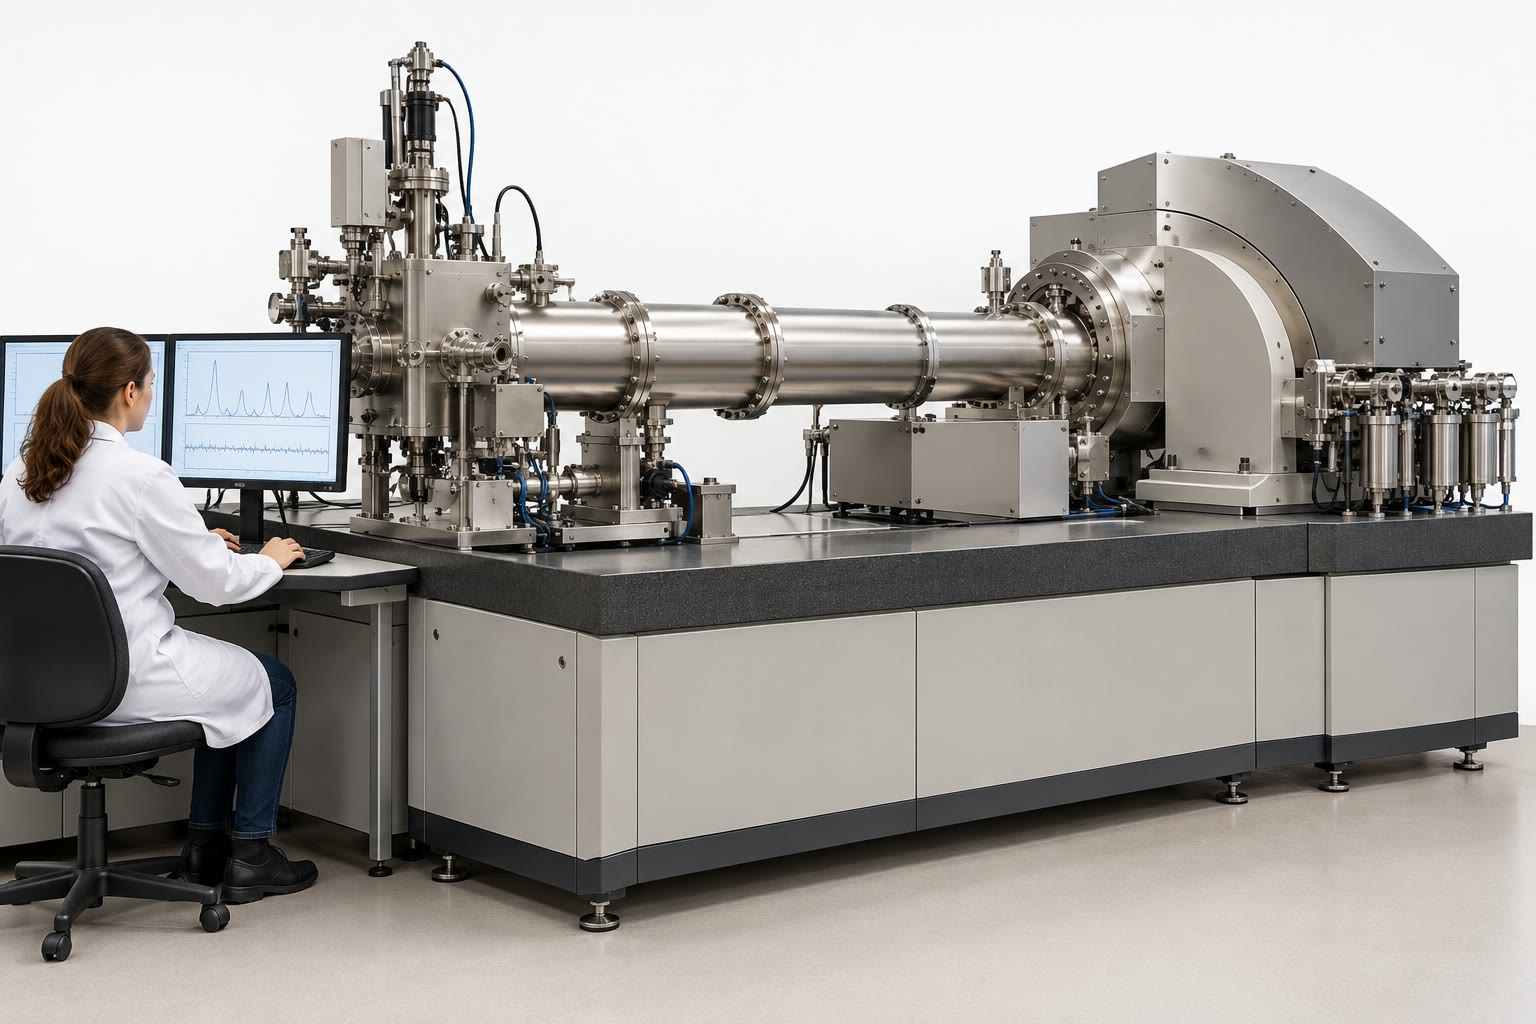
\includegraphics[width=\linewidth]{images/book4/ai/b2-isotope-lab.jpg}
\par\smallskip{\scriptsize Spektrometer massa multikolektor di sebuah laboratorium
isotop (ilustrasi buatan AI).}
\end{minipage}
\end{inthelab}
% ledger: white:chur

\section{Latihan}

\begin{exercise}[$\star$]\label{exo:b2:isotope-geochemistry:1}
Sebuah basal dari Tristan da Cunha memiliki $^{143}\mathrm{Nd}/^{144}\mathrm{Nd} = 0.51249$ dan
basal dari Mangaia 0.51285. Hitunglah $\varepsilon_{\mathrm{Nd}}$ keduanya dan juga nilai untuk
MORB rata-rata (0.513074). Sumber mana yang pernah memiliki Sm/Nd lebih tinggi daripada \omterm{def:b2:planet-formation-meteorites:chondrule}{kondrit}?
\end{exercise}

\begin{exercise}[$\star$]\label{exo:b2:isotope-geochemistry:2}
Perbandingan $^{18}\mathrm{O}/^{16}\mathrm{O}$ bernilai \num{2.0052e-3} pada \omterm{def:b2:isotope-geochemistry:standards}{VSMOW} dan
\num{2.0672e-3} pada \omterm{def:b2:isotope-geochemistry:standards}{VPDB}. Berapa $\delta^{18}\mathrm{O}$ \omterm{def:b2:isotope-geochemistry:standards}{VPDB} pada skala
\omterm{def:b2:isotope-geochemistry:standards}{VSMOW}? Sebuah kalsit memiliki $\delta^{18}\mathrm{O} = -2.0$ permil (\omterm{def:b2:isotope-geochemistry:standards}{VPDB}); hitunglah perbandingannya
dan $\delta^{18}\mathrm{O}$-nya pada skala \omterm{def:b2:isotope-geochemistry:standards}{VSMOW}.
\end{exercise}

\begin{exercise}[$\star$]\label{exo:b2:isotope-geochemistry:3}
Hitunglah $^{143}\mathrm{Nd}/^{144}\mathrm{Nd}$ CHUR \qty{1.0}{Ga} yang lalu dan
\qty{4.567}{Ga} yang lalu ($\lambda_{147} = \qty{6.524e-12}{\per\year}$,
$^{147}\mathrm{Sm}/^{144}\mathrm{Nd} = 0.1966$, saat ini 0.512638).
\end{exercise}

\begin{exercise}[$\star$]\label{exo:b2:isotope-geochemistry:4}
Sebuah sampel salju dari stasiun pegunungan memiliki $\delta^{18}\mathrm{O} = -18.0$ permil.
Berapa $\delta\mathrm{D}$ yang diramalkan \omterm{prop:b2:isotope-geochemistry:mwl}{garis air meteorik}? Sebuah air danau memiliki
$\delta^{18}\mathrm{O} = -4.0$ dan $\delta\mathrm{D} = -42$ permil: hitunglah kelebihan
deuteriumnya $d = \delta\mathrm{D} - 8\delta^{18}\mathrm{O}$, dan katakan apakah air itu terletak di atas atau
di bawah garis.
\end{exercise}

\begin{exercise}[$\star\star$]\label{exo:b2:isotope-geochemistry:5}
Hitunglah $Q$ pada proposisi pertumbuhan linear. Sebuah granit memiliki Sm \qty{6.0}{ppm}
dan Nd \qty{30}{ppm} (CI: 0.145 dan \qty{0.457}{ppm}). Hitunglah
$f_{\mathrm{Sm/Nd}}$-nya, dan perubahan $\varepsilon_{\mathrm{Nd}}$-nya selama
\qty{500}{Ma}.
\end{exercise}

\begin{exercise}[$\star\star$]\label{exo:b2:isotope-geochemistry:6}
Sebuah kerak terpisah \qty{2.7}{Ga} yang lalu dari mantel dengan
$\varepsilon_{\mathrm{Nd}} = +3.5$, dengan $f_{\mathrm{Sm/Nd}} = -0.45$. Taksirlah
$\varepsilon_{\mathrm{Nd}}$-nya saat ini dengan proposisi pertumbuhan linear. Perhitungan
eksak memberikan $-27.3$; berapa selisih pendekatan itu, dan mengapa pendekatan itu
terlalu tinggi atau terlalu rendah?
\end{exercise}

\begin{exercise}[$\star\star$]\label{exo:b2:isotope-geochemistry:7}
Sebuah magma basal (Sr \qty{130}{ppm}, $^{87}\mathrm{Sr}/^{86}\mathrm{Sr} = 0.7030$)
mengasimilasi granit (Sr \qty{320}{ppm}, 0.7200). Hitunglah
$^{87}\mathrm{Sr}/^{86}\mathrm{Sr}$ campuran dengan 5, 10, dan 20 persen granit.
Tunjukkan bahwa $^{87}\mathrm{Sr}/^{86}\mathrm{Sr}$ berupa garis lurus terhadap $1/\mathrm{Sr}$,
dan berikan kemiringan serta titik potongnya.
\end{exercise}

\begin{exercise}[$\star\star$]\label{exo:b2:isotope-geochemistry:8}
Dengan faktor fraksinasi cair--uap 1.0098 ($^{18}$O) dan 1.084 (D) pada
\qty{20}{\degreeCelsius}, hitunglah $\delta^{18}\mathrm{O}$ dan $\delta\mathrm{D}$
uap yang berada dalam kesetimbangan dengan air samudra (0, 0), serta kemiringan
$\delta\mathrm{D}/\delta^{18}\mathrm{O}$ garis dari air ke uap. Ulangi
pada \qty{0}{\degreeCelsius} (1.0117 dan 1.111). Bandingkan dengan \omterm{prop:b2:isotope-geochemistry:mwl}{garis air meteorik}.
\end{exercise}

\begin{exercise}[$\star\star$]\label{exo:b2:isotope-geochemistry:9}
Kerak benua merupakan 0.51 persen massa Bumi silikat dan memuat,
rata-rata, \qty{27}{ppm} Nd dibandingkan \qty{1.25}{ppm} untuk Bumi silikat. Ambillah
$\varepsilon_{\mathrm{Nd}}$ kerak $-15$ dan nilai untuk Bumi silikat 0. Berapa
bagian neodimium yang dimuat kerak? Jika sisa mantel seragam,
berapa $\varepsilon_{\mathrm{Nd}}$-nya? Berapa bagian neodimium yang harus dimuat
reservoir terkuras pada $+8.5$ jika sisa mantel kondritik?
\end{exercise}

\begin{exercise}[$\star\star\star$]\label{exo:b2:isotope-geochemistry:10}
Tunjukkan bahwa dalam proposisi pertumbuhan linear suku-suku yang diabaikan berukuran relatif
sekitar $\lambda t/2$. Sepanjang umur Bumi, seberapa besar nilai ini, dan seberapa
besar galat yang ditimbulkannya pada $\varepsilon_{\mathrm{Nd}}$ untuk $f = -0.45$ selama
\qty{2.7}{Ga}?
\end{exercise}

\begin{exercise}[$\star\star\star$]\label{exo:b2:isotope-geochemistry:11}
Dua komponen memiliki perbandingan Sr/Nd 13.3 (A) dan 5.0 (B). Dengan bukti
\omterm{prop:b2:isotope-geochemistry:mixing}{hiperbola pencampuran}, tentukan bagian $s'$ stronsium dari A dalam campuran yang A-nya
menyumbang bagian $s = 0.5$ neodimium. Untuk nilai $s$ berapa kedua
bagian itu paling berbeda?
\end{exercise}

\begin{exercise}[$\star\star\star$]\label{exo:b2:isotope-geochemistry:12}
Sebuah model kotak memberikan 2.3 hingga 2.6 kali volume kerak benua saat ini,
\qty{7.2e9}{km^3}, dibentuk sejak Bumi terbentuk \qty{4.5}{Ga} yang lalu, dan 1.3 hingga 1.6
kali dihancurkan. Hitunglah laju rata-rata pembentukan dan penghancuran dalam
\unit{km^3} per tahun. Bandingkan dengan laju saat ini di zona subduksi,
\qty{2.7}{km^3} per tahun ditambahkan dan \qty{3.2}{km^3} per tahun disingkirkan.
\end{exercise}

\section{Soal: Tiga pulau, tiga mantel}

\begin{problem}[{Soal akhir pekan --- menempatkan lava tiga pulau pada
larik mantel, memisahkan campuran dari komponen ketiga, dan menentukan umur
sedimen yang didaur ulang}]
\label{pb:b2:isotope-geochemistry:1}
Tiga pulau gunung api di sebuah samudra khayalan, Kora, Vel, dan Asha, mengerupsikan basal
dengan perbandingan isotop di bawah ini. Seorang ahli geokimia memodelkan sumbernya dengan dua
komponen: \omterm{def:b2:isotope-geochemistry:reservoirs}{mantel terkuras} seperti sumber MORB (Sr \qty{10}{ppm}, Nd
\qty{0.75}{ppm}, $^{87}\mathrm{Sr}/^{86}\mathrm{Sr} = 0.70282$,
$^{143}\mathrm{Nd}/^{144}\mathrm{Nd} = 0.51307$) dan sedimen tua yang dikembalikan ke
mantel oleh subduksi (Sr \qty{200}{ppm}, Nd \qty{40}{ppm}, $0.72000$, $0.51141$;
$^{147}\mathrm{Sm}/^{144}\mathrm{Nd} = 0.110$, $^{87}\mathrm{Rb}/^{86}\mathrm{Sr} = 0.50$).
Kora: $0.70410$, $0.51278$; Vel: $0.70618$, $0.51242$; Asha: $0.70290$, $0.51288$
($^{87}\mathrm{Sr}/^{86}\mathrm{Sr}$, $^{143}\mathrm{Nd}/^{144}\mathrm{Nd}$). CHUR saat ini:
$^{143}\mathrm{Nd}/^{144}\mathrm{Nd} = 0.512638$, $^{147}\mathrm{Sm}/^{144}\mathrm{Nd} =
0.1966$; $\lambda_{147} = \qty{6.524e-12}{\per\year}$, $\lambda_{87} =
\qty{1.3972e-11}{\per\year}$.

\medskip\noindent\textbf{Bagian I --- Menempatkan pulau-pulau.}
\begin{enumerate}
\item Hitunglah $\varepsilon_{\mathrm{Nd}}$ kedua komponen.
\item Hitunglah $\varepsilon_{\mathrm{Nd}}$ ketiga pulau.
\item Tempatkan kelima komposisi itu pada diagram Sr--$\varepsilon_{\mathrm{Nd}}$. Pulau
mana yang terletak di sisi CHUR yang diperkaya?
\item Asha memiliki perbandingan stronsium yang hampir sama dengan \omterm{def:b2:isotope-geochemistry:reservoirs}{mantel terkuras}, tetapi
$\varepsilon_{\mathrm{Nd}}$ yang jauh lebih rendah. Di mana Asha terplot relatif terhadap larik mantel, dan
kelompok pulau mana pada bab ini yang dimiripinya?
\item Mengapa perbandingan isotop lava dapat dianggap sama dengan perbandingan isotop sumbernya,
meskipun Sm/Nd dan Rb/Sr lava sangat berbeda dari sumbernya?
\item Sebuah lava Kora dengan $^{147}\mathrm{Sm}/^{144}\mathrm{Nd} = 0.12$ berumur \qty{1}{Ma}.
Seberapa besar $^{143}\mathrm{Nd}/^{144}\mathrm{Nd}$-nya telah bertambah sejak erupsi, dalam
satuan epsilon? Apakah hal ini penting?
\end{enumerate}

\noindent\textbf{Bagian II --- Mencampur kedua komponen.}
\begin{enumerate}[resume]
\item Tuliskan konsentrasi Nd dan $^{143}\mathrm{Nd}/^{144}\mathrm{Nd}$ sebuah
campuran dengan fraksi massa sedimen $f$.
\item Hitunglah $\varepsilon_{\mathrm{Nd}}$ campuran dengan $f = 0.5$, 1, 2, dan 5
persen.
\item Hitunglah $^{87}\mathrm{Sr}/^{86}\mathrm{Sr}$ campuran-campuran yang sama.
\item Tunjukkan bahwa $^{87}\mathrm{Sr}/^{86}\mathrm{Sr}$ campuran-campuran itu berupa garis
lurus terhadap $1/\mathrm{Sr}$, dan berikan kemiringannya.
\item Hitunglah $K = (\mathrm{Sr}/\mathrm{Nd})_{\text{mantel}}/(\mathrm{Sr}/\mathrm{Nd})_{\text{sedimen}}$.
Perbandingan mana, Sr atau Nd, yang bergerak menuju sedimen lebih cepat ketika $f$ bertambah?
\item Berapa kali sedimen lebih kaya daripada mantel dalam Nd, dan dalam Sr?
Jelaskan dengan angka-angka ini mengapa satu persen sedimen menggeser
$\varepsilon_{\mathrm{Nd}}$ sekitar 11 satuan.
\item Berapa bagian neodimium campuran dengan $f = 1$ persen yang berasal dari
sedimen?
\end{enumerate}

\noindent\textbf{Bagian III --- Berapa banyak sedimen?}
\begin{enumerate}[resume]
\item Selesaikan persamaan pencampuran Nd untuk $f$, jika perbandingan $R$ campuran diketahui.
\item Hitunglah $f$ untuk Kora dari neodimiumnya.
\item Hitunglah $f$ untuk Kora dari stronsiumnya. Apakah keduanya sesuai?
\item Hitunglah $f$ untuk Vel dari neodimiumnya dan dari stronsiumnya.
\item Hitunglah $f$ untuk Asha dari neodimiumnya, dan perbandingan stronsium yang diramalkan
oleh $f$ ini. Bandingkan dengan nilai terukur: apa kesimpulanmu tentang
sumber Asha?
\item Usulkan komponen ketiga untuk Asha, dari bab ini, dan
perbandingan induk--anak yang pasti dimilikinya.
\end{enumerate}

\noindent\textbf{Bagian IV --- Umur sedimen.}
\begin{enumerate}[resume]
\item Sedimen itu tersubduksi \qty{2.0}{Ga} yang lalu dan sejak itu tertutup.
Hitunglah $^{143}\mathrm{Nd}/^{144}\mathrm{Nd}$-nya, nilai untuk CHUR, dan
$\varepsilon_{\mathrm{Nd}}$-nya pada waktu itu.
\item Ulangi perhitungan itu dengan proposisi pertumbuhan linear.
\item Hitunglah $^{87}\mathrm{Sr}/^{86}\mathrm{Sr}$ sedimen \qty{2.0}{Ga} yang lalu.
\item \qty{2.0}{Ga} yang lalu, kerak pada gambar $\varepsilon_{\mathrm{Nd}}$ memiliki
$\varepsilon_{\mathrm{Nd}} \approx -4.7$. Apakah nilai sedimen pada saat subduksi sesuai
dengan asal dari erosi kerak benua semuda itu?
\item Nyatakan fraksi massa sedimen yang didaur ulang dalam sumber pulau yang paling
diperkaya, angka kunci soal ini.
\end{enumerate}
\end{problem}
% ledger: white:chur, villa20:sm147, villa22:rb87, gale13:isotopes
